\documentclass{standalone}
\usepackage{tikz}
\usepackage{amsmath,dsfont,bm}
\usetikzlibrary{arrows.meta, positioning, shapes.geometric, calc,patterns,quotes,decorations.pathreplacing}
\newcommand \thetapi {\bm{\theta}^{\pi}}
\newcommand \thetaVpi {\bm{\theta}^{V^{\pi}}}
\begin{document}
	
	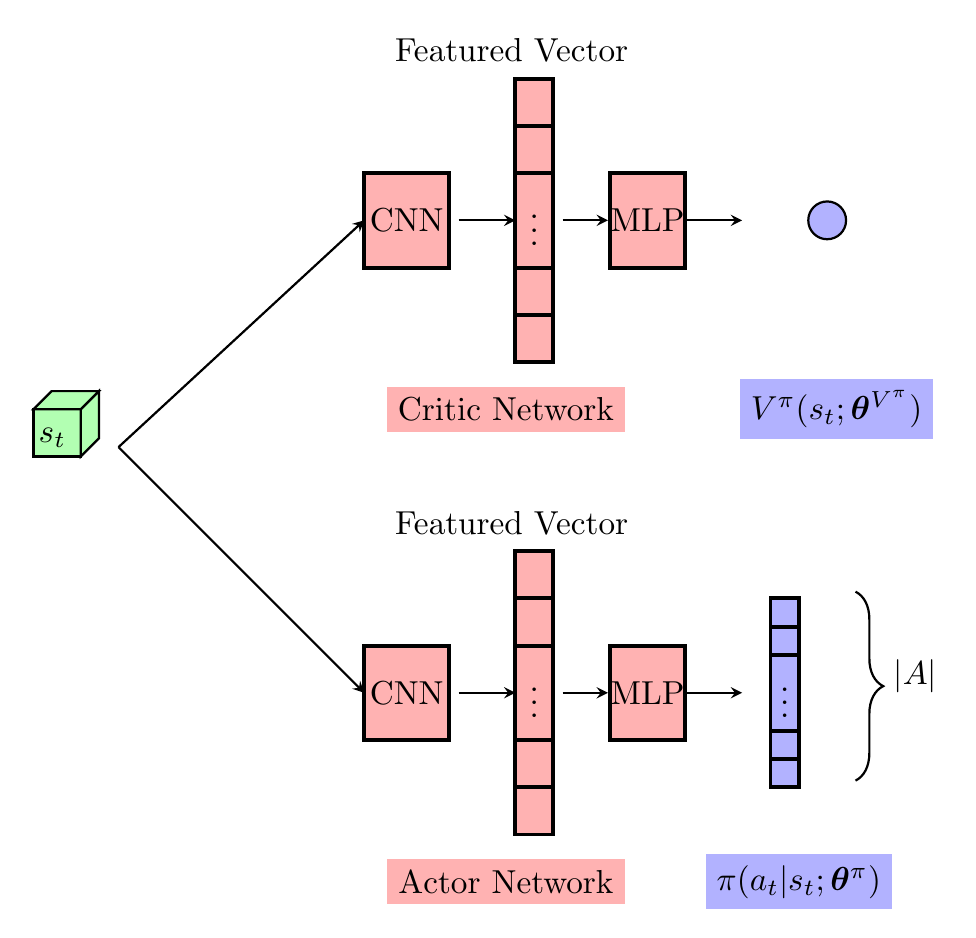
\begin{tikzpicture}[
		thick,scale=1.2, every node/.style={scale=1.2},
		state/.style={draw,circle,pattern=north east lines, pattern color=yellow,radius=0.2},
		action/.style={draw,rectangle, ,pattern=north west lines, pattern color=green}
		]
		
		% Input node (dashed ellipse)
		\pgfmathsetmacro{\cubex}{0.5}
		\pgfmathsetmacro{\cubey}{0.5}
		\pgfmathsetmacro{\cubez}{0.5}
		\draw[black,fill=green!30] (-4,3,0) -- ++(-\cubex,0,0) -- ++(0,-\cubey,0) -- ++(\cubex,0,0) -- cycle;
		\draw[black,fill=green!30] (-4,3,0) -- ++(0,0,-\cubez) -- ++(0,-\cubey,0) -- ++(0,0,\cubez) -- cycle;
		\draw[black,fill=green!30] (-4,3,0) -- ++(-\cubex,0,0) -- ++(0,0,-\cubez) -- ++(\cubex,0,0) -- cycle;
		
		% Hidden layers (rectangles)
		\draw[fill=red!30,line width=0.5mm] (-1,0.5+5) rectangle (-0.1,-0.5+5) node[pos=.5] {CNN};
		\draw[fill=red!30,line width=0.5mm] (0.6,1.5+5) rectangle (1,-1.5+5) node[pos=-0.1] {Featured Vector};
		\foreach \y in {-1.5,-1.0,-0.5,0.5,1.0}
		\draw[fill=red!30,line width=0.5mm] (0.6,1.5+5) rectangle (1,\y+5) ;
		\node (FV) at (0.8, 5) {$\vdots$};
		\draw[fill=red!30,line width=0.5mm] (1.6,0.5+5) rectangle (2.4,-0.5+5) node[pos = 0.5]{MLP};
		
		% Arrows between layers
		\draw[->,>=stealth,thick] (-3.6,2.6) -- (-1,5);
		\draw[->,>=stealth,thick] (-0,5) -- (0.6,5);
		\draw[->,>=stealth,thick] (1.1,5) -- (1.58,5);
		\draw[->,>=stealth,thick] (2.4,5) -- (3,5);
		
		
		
		% Dotted line between layers
		%	\draw[dotted,thick] (0,0) -- (1,0);
		
		% Output arrows
		%	\foreach \y in {1.0, 0.5, -0.5, -1.0}
		%	\draw[->,>=stealth,thick] (3,0) -- (3.5,0);
		
		% Output circles
		%	\foreach \y in {1.0, 0.5, -0.5, -1.0}
		\filldraw[fill=blue!30] (3.9,5) circle [radius=0.2];
		
		% Output label
		%	\node at (3.9, 0.1) {$\vdots$};
		%	\draw [thick, decorate,decoration={brace,amplitude=10pt},yshift=2pt] (4.1,1.5) -- (4.1,-1.5) node [black,midway,xshift = 18pt,yshift=3pt] {$|\mathds{A}|$};
		
		% Network label
		\node [fill = none]at (-4.3,2.7) (st){$s_t$};
		
		
		\node [fill = red!30!] at (0.5, 3)(NN) {Critic  Network };
		
		% V-function label
		\node [fill = blue!30] at (4, -2+5)(Q) {$V^{\pi}(s_t;\thetaVpi)$};
		%	\draw[->,>=stealth,thick](st)--(NN);
		%\draw[->,>=stealth,thick](NN.east)--(Q.west);
		
		
		
		
		
		
		
		
		
		
		
		
		
		%%%% Actor Network
		
		% Hidden layers (rectangles)
		\draw[fill=red!30,line width=0.5mm] (-1,0.5) rectangle (-0.1,-0.5) node[pos=.5] {CNN};
		\draw[fill=red!30,line width=0.5mm] (0.6,1.5) rectangle (1,-1.5) node[pos=-0.1] {Featured Vector};
		\foreach \y in {-1.5,-1.0,-0.5,0.5,1.0}
		\draw[fill=red!30,line width=0.5mm] (0.6,1.5) rectangle (1,\y) ;
		\node (FV) at (0.8, 0) {$\vdots$};
		\draw[fill=red!30,line width=0.5mm] (1.6,0.5) rectangle (2.4,-0.5) node[pos = 0.5]{MLP};
		
		% Arrows between layers
		\draw[->,>=stealth,thick] (-3.6,2.6) -- (-1,0);
		\draw[->,>=stealth,thick] (-0,0) -- (0.6,0);
		\draw[->,>=stealth,thick] (1.1,0) -- (1.58,0);
		\draw[->,>=stealth,thick] (2.4,0) -- (3,0);
		
		
		
		% Dotted line between layers
		%\draw[dotted,thick] (0,0) -- (1,0);
		
		% Output arrows
		%	\foreach \y in {1.0, 0.5, -0.5, -1.0}
		%	\draw[->,>=stealth,thick] (2.2,0) -- (3,\y);
		%	\filldraw[fill=blue!30] (3,0) circle [radius=0.2];
		% Output circles
		%	\foreach \y in {1.0, 0.5, -0.5, -1.0}
		%	\filldraw[fill=blue!30] (3.2,\y) circle [radius=0.2];
		
		% Output label
		%	\node at (3.2, 0.1) {$\vdots$};
		\foreach \y in {-1.0, -0.7,-0.4,0.4, 0.7,1.0}
		\draw[fill=blue!30,line width=0.5mm] (3.3,1) rectangle (3.6,\y) ;
		\node (output) at (3.3+0.15, 0) {$\vdots$};
		
		\draw [thick, decorate,decoration={brace,amplitude=10pt},yshift=2pt] (4.2,1) -- (4.2,-1) node [black,midway,xshift = 18pt,yshift=3pt] {$|\mathds{A}|$};
		% different probabilities
		
		%		\draw[fill=blue!30,draw opacity=0.1] (3.3,1) rectangle ++(0.5,-0.2);
		%		\draw[fill=blue!30,draw opacity=0.1] (3.3,0.7) rectangle++(0.2,-0.2);
		%		\draw[fill=blue!30,draw opacity=0.1] (3.3,0.4) rectangle++(0.7,-0.2);
		%		\draw[fill=blue!30,draw opacity=0.1] (3.3,0.1) rectangle ++(0.8,-0.2);
		%		\draw[fill=blue!30,draw opacity=0.1] (3.3,-0.2) rectangle ++(0.2,-0.2);
		%		\draw[fill=blue!30,draw opacity=0.1] (3.3,-0.5) rectangle ++(0.1,-0.2);
		% Network label
		%	\node [fill = green!30] at (-2.5,-2) (st){$s_t$};
		
		\node [fill = red!30] at (0.5, -2)(NN) {Actor Network };
		
		% Q-function label
		\node [fill = blue!30] at (3.6, -2)(Q) {$\pi(a_t|s_t;\thetapi)$};
		%		\draw[->,>=stealth,thick](st)--(NN);
		%		\draw[->,>=stealth,thick](NN.east)--(Q.west);
	\end{tikzpicture}
	
\end{document}
